\subsection{Question 3: Texturometry}

Two differences in the mechanical testing methods:
\begin{itemize}
    \item[1.] Rheology measures the flow and deformation of materials under applied stress or strain, while texturometry 
    measures the mechanical properties of materials under compression, tension, or shearing forces.
    \item[2.] Rheology tests are typically performed using a rheometer, which applies precise controlled shear or tensile 
    stresses to the sample and measures the resulting deformation or stress response. Texturometry tests, on the other 
    hand, are performed using a texture analyzer, which applies a compressive, tensile, or shearing force to the sample and measures the resulting deformation or force response.
\end{itemize}

Two researchers performed texturometry tests, and Table \ref{tab:inverted-mechanical-test-results} and \ref{tab:inverted-mechanical-test-results-10wv} show the results of a texture profile analysis (TPA) conducted by researcher 1. Comparing the hardness (ability to resist deformation) and springiness (ability to recover to the original shape after compression) between the two tables indicates that higher w/v\% values result in a stiffer/harder material with a better ability to recover its original shape after compression. Increasing the DS of the GelMA sheet would hypothetically increase its hardness and springiness because a higher DS would allow for more crosslinks, resulting in a more rigid structure.

\begin{table}[ht]
    \centering
    \begin{tabular}{c|ccc}
    \hline
    & Sample 1 & Sample 2 & Sample 3 \\ \hline
    Hardness1 [N] & 0.035167098 & 0.043005662 & 0.04099971 \\ 
    Hardness2 [N] & 0.030627189 & 0.032652594 & 0.040604329 \\ 
    Area1 [Nmm] & 0.003338952 & 0.002307124 & 0.003828073 \\ 
    Area2 [Nmm] & 0.001615961 & 0.000898191 & 0.002239604 \\ 
    Cohesiveness & 0.483972601 & 0.389311989 & 0.585047474 \\ 
    Springiness [mm] & 0.282010363 & 0.218791648 & 0.270347203 \\ 
    Springiness Index & 0.531212397 & 0.402065399 & 0.544778107 \\ 
    Gumminess [N] & 0.017019912 & 0.01674262 & 0.023986777 \\ 
    Chewiness [Nm] & 4.79979E-06 & 3.66315E-06 & 6.48476E-06 \\
    \end{tabular}
    \caption{TPA results - 5 w/v\%}
    \label{tab:inverted-mechanical-test-results}
\end{table}

\begin{table}[ht]
    \centering
    \begin{tabular}{c|ccc}
    \hline
    & Sample 1 & Sample 2 & Sample 3 \\ \hline
    Hardness1 [N] & 0.067449574 & 0.06582288 & 0.072415185 \\ 
    Hardness2 [N] & 0.06262254 & 0.064647785 & 0.067325579 \\ 
    Area1 [Nmm] & 0.007224188 & 0.006074186 & 0.008424538 \\ 
    Area2 [Nmm] & 0.005469138 & 0.004678299 & 0.005826683 \\ 
    Cohesiveness & 0.757059224 & 0.770193572 & 0.691632352 \\ 
    Springiness [mm] & 0.465056416 & 0.38483355 & 0.420807332 \\ 
    Springiness Index & 0.889844319 & 0.767740421 & 0.767942963 \\ 
    Gumminess [N] & 0.051063322 & 0.050696359 & 0.050084685 \\ 
    Chewiness [Nm] & 2.37473E-05 & 1.95097E-05 & 2.1076E-05 \\
    \end{tabular}
    \caption{TPA results - 10 w/v\%}
    \label{tab:inverted-mechanical-test-results-10wv}
\end{table}

The second researcher conducted a fracture test, and the results are shown in Figure \ref{fig:fracture}. The figure shows that higher DS values result in a stiffer material because less deflection is reached before fracture for a higher load. The extension relation is slightly different, as it shows a greater ability to extend for intermediate DS values. As previously discussed, a higher DS results in more crosslinks, making the material stiffer. However, for a very low DS, the structure has too few crosslinks to tolerate high loads, and it breaks earlier than a structure with an intermediate DS. Applying the same logic to the concentration of GelMA used to create the sheet yields similar results as for different DS values. A higher concentration implies more crosslinks, resulting in a stiffer structure, and lower concentrations have the opposite effect. Therefore, for increasing concentrations, the deflection would decrease with increasing load, as well as the extension.

\begin{figure}[H]
    \centering
    \begin{subfigure}[b]{0.45\textwidth}
    \centering
    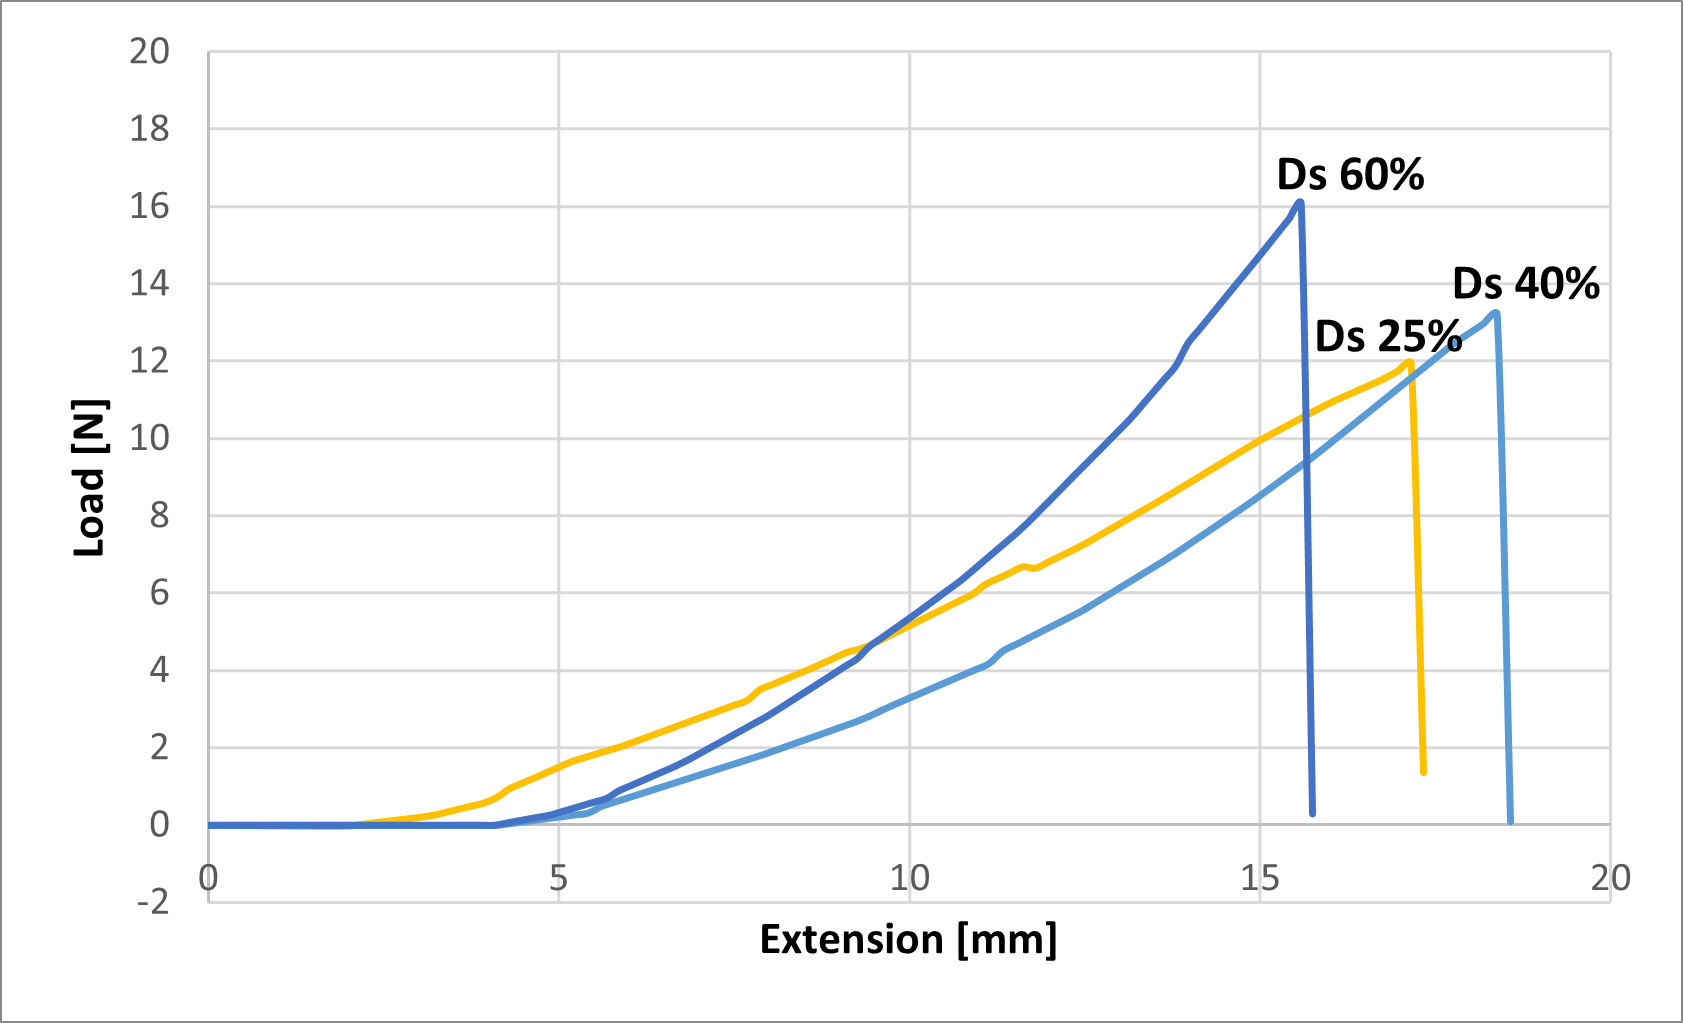
\includegraphics[width=\textwidth]{facture.png}
    \end{subfigure}
    \begin{subfigure}[b]{0.45\textwidth}
    \centering
    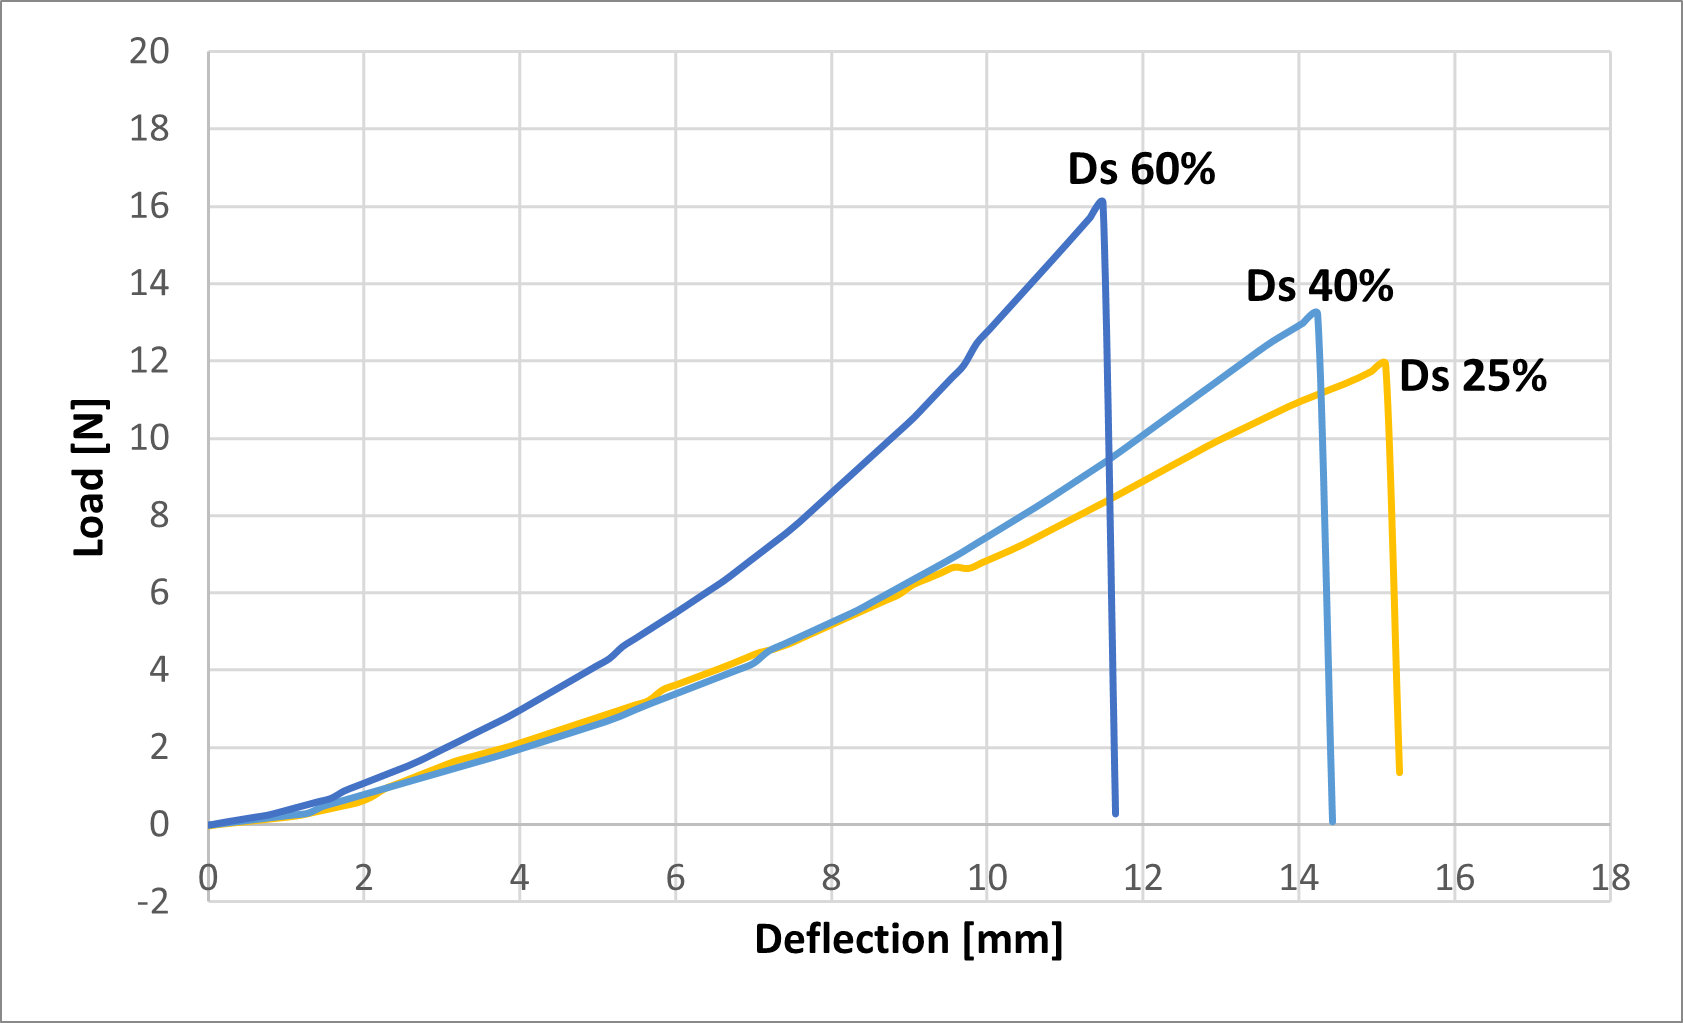
\includegraphics[width=\textwidth]{deflection.png}
    \end{subfigure}
    \caption{Fracture test - load vs extension (left) and load vs deflection (right)}
    \label{fig:fracture}
\end{figure}